\section{Inducción y Recurrencia}
\subsection{Introducción a los naturales}
En el estudio de los números naturales es necesario establecer un punto de partida y a partir de ahí, podremos definir operaciones básicas como la suma, el producto o el orden. Para ello, usaremos de punto de partida los axiomas de Peano y de esta forma llegaremos a todo lo que conocemos sobre los números naturales.
\subsection{Axiomática de Peano}
Supongamos que existe un conjunto $\mathbb{N}$. Los elementos de este conjunto se llaman números naturales.
\begin{ndef}[Axiomas de Peano]
    Los axiomas que definen a $\nat$ son los siguientes:
    \begin{enumerate}[label=\emph{A\arabic*}]
        \item\label{a0} El cero es un número natural. $0 \in \mathbb{N}$
        \item\label{a1} El siguiente de un número natural es un número natural. Si $n \in \mathbb{N} \Rightarrow \sigma(n) \in \mathbb{N}$
        \item\label{a2} Cero no es el siguiente de ningún número natural. $\forall n \in \mathbb{N}$, $\sigma(n) \neq 0$
        \item\label{a3} Si los siguientes de dos números naturales son iguales, entonces los números naturales son iguales. $\forall m,n \in \mathbb{N}, \sigma(n) = \sigma(m) \Rightarrow m = n$
        \item\label{a4} Si un subconjunto de números naturales tiene el cero y siempre que tiene un número tiene a su siguiente, entonces el subconjunto son todos los números naturales.
    \end{enumerate}
\end{ndef}

\begin{nota}
    Podemos definir $\sigma(n) = n + 1$ $\forall n \in \nat$.
\end{nota}

\begin{nth}
    Todo número natural es distinto del siguiente. $\forall n \in \nat n \neq \sigma(n)$
\end{nth}
\begin{proof}
    Sea $A = \{x \in \nat : x \neq \sigma(x)\}$: \\
    Como $0 \neq \sigma(0)$, resulta $0 \in A$.
    Supongamos ahora $n \in A$, es decir, $n \neq \sigma(n)$, luego $\sigma(n) \neq \sigma(\sigma(n))$, por tanto, $\sigma(n) \in A$.
    Luego $A = \nat$.
\end{proof}

\begin{nth}
    Para cada número natural distinto de cero, existe un único número natural del que es su siguiente. $\forall n \in \nat (n \neq 0 \Rightarrow \exists! m \in \nat$ tal que $x = \sigma(m))$
\end{nth}
\begin{proof}
    Sea $A = \{x \in \nat : x = 0$ o $m \in \nat$ tal que $x = \sigma(m)\}$:\\
    Como $0 = 0$, resulta $0 \in A$. Supongamos ahora $n \in A$, es decir, $n = 0$ o $n = \sigma(m)$. En cualquier caso, $\sigma(n) = \sigma(n)$, por tanto $\sigma(n) \in A$. Luego $A = \nat$. \\
    La unicidad es consecuencia de $A4$.
\end{proof}

\subsection{Aritmética natural}
\subsubsection{Suma de naturales}
\begin{nth}
    Existe una única $+ : \nat \times \nat \rightarrow \nat$ tal que $\forall m,n \in \nat$ verifica:
    \begin{itemize}
        \item $m + 0 = m$
        \item $m + \sigma(n) = \sigma(m + n)$
    \end{itemize}
\end{nth}
\begin{properties}
    Para todo $m,n,p \in \nat$ se cumple:
    \begin{enumerate}
        \item Todo número natural es 0 o es el siguiente de un número natural.
        \item $m + 0 = 0 + m = m$.
        \item $m + 1 = 1 + m = \sigma(m)$.
        \item $(m + n) + p = m + (n + p)$.
        \item $m + n = n + m$.
        \item Si $m + p = n + p$, entonces $m = n$.
        \item Si $m + n = 0$, entonces $m = n = 0$.
    \end{enumerate}
\end{properties}

\subsubsection{Producto de naturales}
\begin{nth}
    Existe una única $\cdot : \nat \times \nat \rightarrow \nat$ tal que $\forall m,n \in \nat$ verifica:
    \begin{itemize}
        \item $m \cdot 0 = 0$
        \item $m \cdot \sigma(n) =  m \cdot n + m$
    \end{itemize}
\end{nth}

\begin{properties}
    Para todo $m,n,p \in \nat$ se cumple:
    \begin{enumerate}
        \item $0 \cdot m = m \cdot 0 = 0$.
        \item $1 \cdot m = m \cdot 1 = m$.
        \item $(m + n) \cdot p = m \cdot p + n \cdot p$.
        \item $m \cdot n = n \cdot m$.
        \item Si $(m \cdot n) \cdot p = m \cdot (n \cdot p)$.
        \item Si $m \cdot n = 0$, entonces $m = 0$ o $n = 0$.
    \end{enumerate}
\end{properties}

\subsubsection{Potencias de naturales}
\begin{nth}
    Existe una única $\square^{\square} : \nat \times \nat \rightarrow \nat$ tal que $\forall m,n \in \nat$ verifica:
    \begin{itemize}
        \item $m^{0} = 1$
        \item $m^{\sigma(n)} =  m^{n} \cdot m$
    \end{itemize}
\end{nth}

\begin{properties}
    Para todo $m,n,p \in \nat$ se cumple:
    \begin{enumerate}
        \item $0^{0} = 1$.
        \item $0^{n} = 0$ para $1 \leq n$.
        \item $1^{n} = 1$.
        \item $m^{n+p} = m^{n} \cdot m^{p}$.
        \item Si $m^{n \cdot p} = (m^{n})^{p}$.
    \end{enumerate}
\end{properties}

\subsubsection{El orden de los naturales}
Primero definamos en qué consiste una relación de orden:
\begin{ndef}
    Sea $(A,R)$ un par ordenado con $A$ un conjunto no vacío y $R$ una relación binaria definida en $A$, entonces se dice que $R$ es una \textbf{relación de orden} si es:
    \begin{itemize}
        \item \textbf{Reflexiva}: Todo elemento de $A$ A está relacionado consigo mismo. Es decir, $\forall x\in A,\ xRx$.
        \item \textbf{Antisimétrica}: Si dos elementos de $A$ se relacionan entre sí, entonces ellos son iguales. Es decir, $\forall x,y\in A,\ xRy,\ yRx \ \Rightarrow \ x=y$.
        \item \textbf{Transitiva}: Si un elemento de $A$ está relacionado con otro, y ese otro a su vez se relaciona con un tercero, entonces el primero estará relacionado también con este último. Es decir, $\forall x,y,z\in A,\;xRy,yRz\Rightarrow xRz$.
    \end{itemize}
\end{ndef}
\begin{ndef}[Orden]
    Dados $m,n \in \nat$ definimos m es menor o igual que n $(m \leq n)$ si $\exists x \in \nat$ tal que $m + x = n$. Lo podemos representar como $(\nat,\leq)$.
\end{ndef}

\begin{properties}
    Para todo $m,n,p \in \nat$ se cumple:
    \begin{enumerate}
        \item $m \leq m$.
        \item Si $m \leq n$ y $n \leq m$, entonces $m = n$.
        \item Si $m \leq n$ y $n \leq p$, entonces $m \leq p$.
        \item $m \leq n$ o $n \leq m$.
        \item Si $m \leq n$, entonces $\exists! p \in \nat$ tal que $m + p = n$ y lo llamamos n menos m $(n - m)$.
        \item Si $m \leq n$, entonces $m + p \leq n + p$.
        \item Si $m \leq n$, entonces $m \cdot p \leq n \cdot p$.
        \item Si $m \cdot p \leq n \cdot p$ y $p \neq 0$, entonces $m \leq n$.
        \item Si $m \cdot p = n \cdot p$ y $p \neq 0$, entonces $m = n$.
    \end{enumerate}
\end{properties}

\subsubsection{Divisibilidad en $\nat$}
\begin{ndef}[Divisibilidad]
    Dados $m,n \in \nat$ definimimos m divide a n $(m|n)$ si $\exists x \in \nat$ tal que $m \cdot x = n$.
\end{ndef}

\begin{properties}
    Para todo $m,n,p \in \nat$ se cumple:
    \begin{enumerate}
        \item $m|m$.
        \item Si $m|n$ y $n|m$, entonces $m = n$.
        \item Si $m|n$ y $n|p$, entonces $m|p$.
        \item Si $m|n$, entonces $\exists! p \in \nat$ tal que $m \cdot p = n$ y lo llamamos n partido por m $\left( \frac{n}{m} \right)$.
    \end{enumerate}
\end{properties}

\subsection{Principio de inducción}
\begin{nth}
    Las tres propiedades que siguen son equivalentes:
    \begin{enumerate}
        \item \textbf{Principio de inducción}. Si $A \subseteq \nat$ cumple $0 \in A$ y $(n \in A \Rightarrow n + 1 \in A)$, entonces $A = \nat$.
        \item \textbf{Principio del buen orden}. Todo subconjunto no vacío de números naturales tiene mínimo.
        \item \textbf{Principio de inducción completa}. Si $A \subseteq \nat$ cumple $0 \in A$ y si $(\{0,1,...,n\} \subseteq A \Rightarrow n + 1 \in A)$, entonces $A = \nat$.
    \end{enumerate}
\end{nth}

\subsection{Ecuaciones en recurrencia}
\begin{ndef}
    Una \textbf{ecuación en recurrencia} es un tipo específico de relación de recurrencia. Una relación de recurrencia es una sucesión $\{a_{n}\}$ que relaciona $a_{n}$ con
    alguno de sus predeesores $a_{0}$, $a_{1}, \ldots , a_{n-1}$ para $n \in \nat$. Las condiciones iniciales para la sucesión $\{a_{n}\}$ son valores dados en forma explícita
    para un número finito de términos de la sucesión.
\end{ndef}
\begin{ejemplo}
    Número de regiones del plano determinadas por $n$ rectas no paralelas y que por cualquier punto del plano pasan como máximo dos de ellas.
    \\
    Condiciones iniciales: $a_{1} = 2$, $a_{2} = 4$, $a_{3} = 7$, $a_{4} = 11$.
    \begin{center}
        $a_{n} = a_{n-1} + n$  para  $2 \leq n$
    \end{center}
\end{ejemplo}

\begin{ejemplo}
    Torres de Hanoi.
    \\
    Condiciones iniciales: $a_{1} = 1.$
    \begin{center}
        $a_{n} = 2a_{n-1} + 1$  para  $2 \leq n$
    \end{center}
\end{ejemplo}

\begin{ejemplo}
    Llamemos $a_{n}$ al número de listas de longitud $n$ formadas con ceros y unos que no tienen unos consecutivos.
    \\
    Condiciones iniciales: $a_{1} = 2$, $a_{2} = 3.$
    \begin{center}
        $a_{n} = a_{n-1} + a_{n-2}$  para  $3 \leq n$
    \end{center}
\end{ejemplo}

\begin{ejemplo}
    Sucesión de Fibonacci.
    \\
    Condiciones iniciales: $F_{1} = 0$, $F_{2} = 1.$
    \begin{center}
        $F_{n} = F_{n-1} + F_{n-2}$  para  $3 \leq n$
    \end{center}
\end{ejemplo}

\subsubsection{Recurrencias homogéneas}
\begin{ndef}
    Sea $x: \nat \rightarrow \mathbb{R}$ una sucesión. Decimos que dicha sucesión satisface una \textbf{relación de recurrencia lineal homogénea con coeficientes constantes}
    si existe $ k \in \nat, \ a_1, \dots$ y $a_k \in \mathbb{R}$ tales que para cualquier $n \geq k$ se verifica que
    $\sum_{j=0}^k a_j \cdot x_{n-j} = a_0 \cdot x_n + a_1 \cdot x_{n-1} + \ldots + a_k \cdot x_{n-k} = 0$,
    donde $a_0 = 1$.
    Al número $k$ se le denomina orden de la relación.
\end{ndef}


Las \textbf{condiciones iniciales} son los $k$ términos de la sucesión de la relación de recurrencia que son necesarios para poner en funcionamiento la recurrencia de orden $k$.
Nuestro objetivo es hallar dicha sucesión que satisfaga la relación, siendo esta situación un \textbf{problema de recurrencia} y cada una de las sucesiones son las \textbf{soluciones del problema de recurrencia}.


\begin{ndef}
    Dado un problema de recurrencia lineal homogénea con coeficientes constantes $x_n + a_1x_{n-1} + \ldots + a_kx_{n-k} = 0$. Al polinomio
    $x^k + a_1x^{k-1} + \ldots + a_{k-1}x + a_k$ se le conoce como \textbf{polinomio característico de la relación}, y a la ecuación
    $x^k + a_1x^{k-1} + \ldots + a_{k-1}x + a_k = 0$ la \textbf{ecuación característica}.
\end{ndef}

\begin{nprop}
    Si $\alpha$ es una solución de la ecuación característica de un problema de recurrencia, entonces la sucesión $x_n = \alpha^n$ es una solución a dicho problema.
\end{nprop}

Cabe destacar que si $\alpha_1, \alpha _2, \ldots, \alpha_k$ son raíces del polinomio característico de una relación de recurrencia con $\alpha_i \neq \alpha_j \ \forall i,j < k $ con $i \neq j$,
entonces $x_n = b_1\alpha_1^n + b_2\alpha_2^n + \ldots + b_k\alpha_k^n$ es solución de la relación de equivalencia, siendo las condiciones iniciales las que determinan $b_1, b_2, \ldots, b_k$.


\begin{nprop}
    Sea  $x_n + a_1x_{n-1} + \ldots + a_kx^{n-k}$ un problema de recurrencia, $p(x)$ su polinomio característico y $\alpha$ una raíz doble de $p(x)$, entonces
    $x_n = \alpha^n$ es una solución a dicho problema.
\end{nprop}

\begin{ejemplo}[Raíces simples] $a_{n} + a_{n-1} -6a_{n-2} = 0$ para $n \geq 2$ \\
    Condiciones iniciales: $a_{0} = 1$, $a_{1} = 2$.\\
    Hallamos el polinomio característico y factorizamos: $x^2 + x -6 = (x-2)(x+3)$\\
    Solución general: $s_{n} = A \cdot 2^{n} + B \cdot (-3)^{n}$ \\
    Solución particular: la hallamos resolviendo el sistema dado por las condiciones iniciales:
    \begin{center}
        $\left.
            \begin{aligned}
                1 = A + B \\
                2 = 2A - 3B
            \end{aligned} \right \}
            \Rightarrow A = -1, \ B = 5 \text{ de donde } a_n = 2^n$
    \end{center}
\end{ejemplo}
\smallskip

\begin{ejemplo}[Raíz doble] $a_{n} - 6a_{n-1} +9a_{n-2} = 0$ para $n \geq 2$ \\
    Condiciones iniciales: $a_{0} = 5$, $a_{1} = 12$.\\
    Hallamos el polinomio característico y factorizamos: $x^2 - 6x + 9 = (x-3)^2$\\
    Solución general: $s_n = (A \cdot n + B) \cdot 3^n$ \\
    Solución particular:
    \begin{center}
        $\left.
            \begin{aligned}
                5 = B \\
                12 = (A + B) \cdot 3
            \end{aligned} \right \}
            \Rightarrow A = -1, \ B = 5 \text{ de donde } a_n = (-n+5) \cdot 3^n$
    \end{center}
\end{ejemplo}
\smallskip

\begin{ejemplo}[Raíces complejas simples] $a_{n} - 2a_{n-1} +2a_{n-2} = 0$ para $n \geq 2$ \\
    Condiciones iniciales: $a_{0} = 0$, $a_{1} = 1$.\\
    Hallamos el polinomio característico y factorizamos: \\ $x^2 - 2x + 2 = (x-(1+i))(x-(1-i))$\\
    Solución general: $s_{n} = A \cdot (1+i)^{n} + B \cdot (1-i)^{n}$ \\
    Solución particular:
    \begin{center}
        $\left.
            \begin{aligned}
                0 = A + B \\
                1 = (1+i)\cdot A - (1-i)\cdot B
            \end{aligned} \right \}
            \Rightarrow A = \cfrac{-i}{2} , \ B = \cfrac{i}{2}  \text{ de donde }  a_n = \cfrac{-i}{2}((1+i)^n -(1-i)^n)$
    \end{center}
\end{ejemplo}
\smallskip

\begin{ejemplo}[Raíces polinomio de grado k] $a_{n} - 5a_{n-1} +8a_{n-2} -4a_{n-3} = 0$ para $n \geq 3$ \\
    Condiciones iniciales: $a_{0} = 0$, $a_{1} = 1$, $a_2 = 2$.\\
    Hallamos el polinomio característico y factorizamos: $x^3 -5x^2 - 2x + 2 = (x-1)(x-2)^2$\\
    Solución general: $s_{n} = A + (B \cdot n + C) \cdot 2^n$ \\
    Solución particular:
    \begin{center}
        $\left.
            \begin{aligned}
                0 = A + C       \\
                1 = A + 2B + 2C \\
                2 = A + 8B + 4C
            \end{aligned} \right \}
            \Rightarrow A = -2 , \ B = -\cfrac{1}{2}, C = 2  \text{ de donde } a_n = -2 + (-\cfrac{1}{2}n + 2) \cdot 2^n$
    \end{center}
\end{ejemplo}
\smallskip

\subsubsection{Recurrencias no homogéneas}
\begin{ndef}
    Sea $x: \nat \rightarrow \mathbb{R}$ una sucesión. Decimos que dicha sucesión satisface una \textbf{relación de recurrencia lineal con coeficientes constantes}
    si existe $ k \in \nat, \ a_1, \dots , a_k \in \mathbb{R}$ y $f:\nat \rightarrow \mathbb{R}$ tales que para cualquier $n \geq k$ se verifica que
    $\sum_{j=0}^k a_j \cdot x_{n-j} = a_0 \cdot x_n + a_1 \cdot x_{n-1} + \ldots + a_k \cdot x_{n-k} = f(n)$,
    donde $a_0 = 1$.
    Al número $k$ se le denomina orden de la relación.
\end{ndef}

\begin{nprop}
    Sea $x_n + a_1x_{n-1} + \ldots + a_kx_{n-k} = f(n)$ un problema de recurrencia lineal no homogénea.
    \begin{itemize}
        \item Supongamos que $u_n$ y $v_n$ son soluciones al problema no homogéneo. Entonces la sucesión $u_n - v_n$ es una solución al problema de recurrencia lineal homogéneo asociado.
        \item Si $y_n$ es una solución al problema no homogéneo, entonces todas las soluciones de dicho problema son de la forma $y_n + h_n$, donde $h_n$ es una solución al problema homogéneo.
    \end{itemize}
\end{nprop}

\begin{nprop}
    Supongamos que $x_n$ es una sucesión que satisface una relación de recurrencia lineal no homogénea
    $x_n + a_1x_{n-1} + \ldots + a_kx_{n-k} = f(n)$ donde $f(n)$ es un polinomio de grado $r$. Entonces $x_n$ satisface una relación de recurrencia lineal homogénea cuyo polinomio característico es
    $(x^k + a_1x^{k-1} + \ldots + a_k)(x - 1)^{r+1}$.
\end{nprop}

De manera similar, la siguiente proposición dice así:
\begin{nprop}
    Supongamos que $x_n$ es una sucesión que satisface una relación de recurrencia lineal no homogénea
    $x_n + a_1x_{n-1} + \ldots + a_kx_{n-k} = b^nf(n)$ donde $f(n)$ es un polinomio de grado $r$. Entonces $x_n$ satisface una relación de recurrencia lineal homogénea cuyo polinomio característico es
    $(x^k + a_1x^{k-1} + \ldots + a_k)(x - b)^{r+1}$.
\end{nprop}

\begin{ejemplo}[Torres de Hanoi] $a_{n} = 2a_{n-1} + 1$ para $n \geq 2$ \\
    Condiciones iniciales: $a_{1} = 1$.\\
    Término no homogéneo: $1 = b^np(n) \implies b = 1, \ p(n) = 1, \ gr(p) = 0$ \\
    Hallamos el polinomio característico (que tiene las soluciones de la ecuación dada y muchas más) y factorizamos: $x^2 -3x + 2 = (x-1)(x-2)$\\
    Solución general(ísima) de una homogénea asociada: $g_{n} = A \cdot 2^n + B$ \\
    Extendemos las soluciones iniciales: $a_1 = 1, \ a_2 = 2a_1 +1 = 2 + 1 = 3$ \\
    Solución particular:
    \begin{center}
        $\left.
            \begin{aligned}
                1 = 2A + B \\
                3 = 4A + B
            \end{aligned} \right \}
            \Rightarrow A = 1 , \ B = -1 \text{ de donde } a_n = 2^n - 1$
    \end{center}
    Extendemos las condiciones iniciales para una sucesión arbitraria: $a_1 = a, \ a_2 = 2a_1 + 1 = 2a + 1$ \\
    Solución general  de la no homogénea:
    \begin{center}
        $\left.
            \begin{aligned}
                a = 2A + B \\
                2a + 1 = 4A + B
            \end{aligned} \right \}
            \Rightarrow A = \cfrac{a+1}{2}, \ B = -1 \text{ de donde } s_n = \cfrac{a+1}{2}2^n - 1$
    \end{center}
\end{ejemplo}
\smallskip

\begin{ejemplo}[Regiones del Plano] Las regiones del plano generadas por $n$ rectas no paralelas y cuyas intersecciones no son de más de dos rectas:
    $a_{n} = 2a_{n-1} + n$ para $n \geq 1$ \\
    Condiciones iniciales: $a_{0} = 1$.\\
    Término no homogéneo: $1 = b^np(n) \implies b = 1, \ p(n) = n, \ gr(p) = 1$ \\
    Hallamos el polinomio característico (que tiene las soluciones de la ecuación dada y muchas más) y factorizamos: $x^3 -3x^2 +3x -1 = (x-1)(x-1)^2$\\
    Solución general(ísima) de una homogénea asociada: $g_{n} = An^2 + Bn + C$ \\
    Extendemos las soluciones iniciales: $a_0 = 1, \ a_1 = a_0 +1 = 2, \ a_2 = a_1 +2 = 4$ \\
    Solución particular:
    \begin{center}
        $\left.
            \begin{aligned}
                1 = C \\
                2 = A + B + C \\
                4 = 4A + 2B + C
            \end{aligned} \right \}
            \Rightarrow A = \cfrac{1}{2}, \ B = \cfrac{1}{2}, \ C = 1 \text{ de donde } a_n = \cfrac{n^2+n+2}{2}$
    \end{center}
    Extendemos las condiciones iniciales para una sucesión arbitraria: $a_0 = a, \ a_1 = a_1 + 1 = a + 1, \ a_2 = a_1 + 2 = a + 3$ \\
    Solución general  de la no homogénea:
    \begin{center}
        $\left.
            \begin{aligned}
                a = C \\
                a + 1 = A + B + C \\
                a + 3 = 4A + 2B + C
            \end{aligned} \right \}
            \Rightarrow A = \cfrac{1}{2}, \ B = \cfrac{1}{2}, \ C = a \text{ de donde } s_n = \cfrac{n^2+n+2a}{2}$
    \end{center}
\end{ejemplo}
\smallskip

Otro tipo de ecuaciones en recurrencia no homogéneas más generales con las que vamos a trabajar son $\sum_{j=0}^k a_jx_{n-j} = a_0x_n + a_1x_{n-1} + \ldots + a_kx_{n-k} = \sum_{i=1}^r b_i^np_i(n)$, para $k \leq n$, 
de donde $a_0, a_1, \cdots, a_k$ son constantes con $a_k \neq 0 \ y \ a_{n-k} \neq 0$, $b_i$ otra constante y $p_i(n)$ un polinomio en $n$ de grado $r_i$.

\begin{ejemplo} $a_{n} = 2a_{n-1} + n + 2^n$ para $n \geq 1$ \\
    Condiciones iniciales: $a_{0} = 0$.\\
    Término no homogéneo: $1 = b^np(n) \implies b = 1, \ p(n) = n, \ gr(p) = 1$ y $2^n = b^np(n) \implies b = 2, \ p(n) = 1, \ gr(p) = 0$ \\
    Hallamos el polinomio característico (que tiene las soluciones de la ecuación dada y muchas más) y factorizamos: $(x-2)(x-1)^2(x-2)$\\
    Solución general(ísima) de una homogénea asociada: $g_{n} = (An + B) \cdot 2^n + Cn + D$ \\
    Extendemos las soluciones iniciales: $a_0 = 0, \ a_1 = 2a_0 +1 +2^1 = 3, \ a_2 = 2a_1 +2 +2^2 = 12, \ a_3 = 2a_2 +3 +2^3 = 35$ \\
    Solución particular:
    \begin{center}
        $\left.
            \begin{aligned}
                0 = B + D \\
                3 = 2A + 2B + C + D \\
                12 = 8A + 4B + 2C + D \\
                35 = 24A + 8B + 3C + D
            \end{aligned} \right \}
            \Rightarrow A = 1, \ B = 2, \ C = -1, \ D = -2 \text{ de donde } a_n = (n+2)\cdot 2^n - (n+2) = (n+2)(2^n-1)$
    \end{center}
    Extendemos las condiciones iniciales para una sucesión arbitraria: $a_0 = a, \ a_1 = 2a_0 +1 +2^1 = 2a+3, \ a_2 = 2a_1 +2 +2^2 = 4a+12, \ a_3 = 2a_2 +3 +2^3 = 8a+35$ \\
    Solución general  de la no homogénea:
    \begin{center}
        $\left.
            \begin{aligned}
                a = B + D \\
                2a+3 = 2A + 2B + C + D \\
                4a+12 = 8A + 4B + 2C + D \\
                8a+35 = 24A + 8B + 3C + D
            \end{aligned} \right \}
            \Rightarrow A = 1, \ B = a+2, \ C = -1, \ D = -2 \text{ de donde } s_n = (n+a+2)\cdot 2^n - (n+2)$ 
    \end{center}
\end{ejemplo}
\smallskip

\newpage
\section{Álgebras de Boole}
\subsection{Álgebras de Boole}
\begin{ndef}[Álgebra de Boole]
    Un álgebra de Boole es una seis-upla $(A, \lor, \land, \overline{\square}, 0, 1)$ donde A es un conjunto no vacío, $\lor$ y $\land$ son operaciones binarias, $\overline{\square}$ es una operación monaria y
    $0$ y $1$ son elementos de $A$. Además $\forall a,b,c \in A$ se cumple:
    \begin{enumerate}[label=\emph{A\arabic*}]
        \item\label{a0} \textbf{Asociatividad} $a \lor (b \lor c) = (a \lor b) \lor c$, $a \land (b \land c) = (a \land b) \land c$
        \item\label{a1} \textbf{Conmutatividad} $a \lor b = b \lor a$, $a \land b = b \land a$
        \item\label{a2} \textbf{Distributividad} $a \lor (b \land c) = (a \lor b) \land (a \lor c)$, $a \land (b \lor c) = (a \land b) \lor (a \land c)$
        \item\label{a3} \textbf{Complementación} $a \lor \overline{x} = 1$, $a \land \overline{x} = 0$
        \item\label{a4} \textbf{Identidad} $a \lor 0 = a$, $a \land 1 = a$
    \end{enumerate}
\end{ndef}
La siguiente definición es equivalente a la anterior:
\begin{ndef}[Huntington]
    Un álgebra de Boole es una seis-upla $(A, \lor, \land, \overline{\square}, 0, 1)$ donde A es un conjunto no vacío, $\lor$ y $\land$ son operaciones binarias, $\overline{\square}$ es una operación monaria y
    $0$ y $1$ son elementos de $A$. Además $\forall a,b,c \in A$ se cumple:
    \begin{enumerate}[label=\emph{A\arabic*}]
        \item\label{a1} \textbf{Conmutatividad} $a \lor b = b \lor a$, $a \land b = b \land a$
        \item\label{a2} \textbf{Distributividad} $a \lor (b \land c) = (a \lor b) \land (a \lor c)$, $a \land (b \lor c) = (a \land b) \lor (a \land c)$
        \item\label{a3} \textbf{Complementación} $a \lor \overline{a}  = 1$, $a \land \overline{a}  = 0$
        \item\label{a4} \textbf{Identidad} $a \lor 0 = a$, $a \land 1 = a$
    \end{enumerate}
\end{ndef}
\begin{nota}
    Los álgebras de Boole cumplen el \textbf{principio de dualidad}, pues si tomamos un axioma y cambiamos $\lor$ por $\land$, $0$ por $1$ y el $1$ por $0$, obtenemos otro axioma. Además,
    si un teorema es cierto para un álgebra de Boole, también lo es para su dual.
\end{nota}

\begin{obs}
    Los símbolos para operaciones de un álgebra de Boole también se suelen notar de distintas formas:
    \begin{itemize}
        \item $\lor$: $+$, OR.
        \item $\land$: $\cdot$, $\times$, AND.
        \item $\overline{\square}$: $\square^*$, $\neg \square$, $\square'$, NOT $\square$.
        \item $0$: F (Falso), F (False).
        \item $1$: V (Verdadero), T (True).
    \end{itemize}
\end{obs}

\begin{properties}
    Supongamos que $(B, \lor, \land, \overline{\square}, 0, 1)$ es un álgebra de Boole y $x,y,z \in B$. Entonces:
    \begin{enumerate}
        \item \textbf{Idempotencia: } $x \lor x = x$; $x \land x = x$.
        \item \textbf{Dominación: } $x \lor 1 = 1$; $x \land 0 = 0$.
        \item \textbf{Absorción: } $x \lor (x \land y) = x$; $x \land (x \lor y) = x$.
        \item \textbf{Propiedad cancelativa: }
              $\left.
                  \begin{aligned}
                      x \lor y = x \lor z, \
                      x \land y = x \land z
                  \end{aligned}
                  \right \} \Rightarrow y = z$
        \item \textbf{Doble complementación: } $\overline{\overline{x}}=x $.
        \item $x \lor (\overline{x}  \land y) = x \lor y$; $x \land (\overline{x} \lor y) = x \land y$.
        \item \textbf{Leyes de De Morgan: } $\overline{x \lor y} = \overline{x} \land \overline{y}$; $\overline{x \land y} = \overline{x} \lor \overline{y}$.
        \item Son equivalentes: $x \lor y = y$, $x \land y = x$, $\overline{x} \lor y = 1$, $x \land \overline{y} = 0$.
    \end{enumerate}
\end{properties}

\begin{nprop}
    Sean $(B_1, \lor_1, \land_1, \overline{\square}, 0, 1)$ y $(B_2, \lor_2, \land_2, \overline{\square}, 0, 1)$ dos álgebras de Boole. Entonces el conjunto $B_1 \times B_2$ con las operaciones
    $(x,y) \lor (x',y') = (x \lor_1 x', y \lor_2 y')$ tiene estructura de álgebra de Boole para $x,x' \in B_1, \ y,y' \in B_2$.
\end{nprop}
\begin{nota}
    Esta proposición es fácilmente extensible por inducción a $B_1 \times B_2 \times \cdots \times B_n$ siendo $B_n$ conjuntos con estructuras de álgebras de Boole.
\end{nota}

\begin{ejemplo}
    Sea $\mathbb{B} = \{ 0,1 \}$. Este conjunto tiene estructura de álgebra de Boole con las operaciones $\lor$ y $\land$ de la forma $(B, \lor, \land, \overline{\square}, 0, 1)$: \\
    \begin{center}
        \begin{tabular}{ll}
            \begin{tabular}{ |c||c|c|  }
                \hline
                $\lor$ & 0 & 1 \\
                \hline
                0      & 0 & 1 \\
                \hline
                1      & 1 & 1 \\
                \hline
            \end{tabular}
            \quad
            \begin{tabular}{ |c||c|c|  }
                \hline
                $\land$ & 0 & 1 \\
                \hline
                0       & 0 & 0 \\
                \hline
                1       & 0 & 1 \\
                \hline
            \end{tabular}
        \end{tabular}
    \end{center}
    mientras que $\overline{0} = 1$ y $\overline{1} = 0$. Luego por la proposición anterior, sabemos que $(\mathbb{B} \times \mathbb{B}, \lor, \land)$ es también un álgebra de Boole.
    De hecho, $\mathbb{B}^n \ \forall n \in \nat$ son álgebras de Boole.
\end{ejemplo}

\begin{nth}[Orden]
    Sea $(B, \lor, \land)$ un álgebra de Boole. Definimos la \textbf{relación de orden en $B$} como: $x \leq y \Longleftrightarrow x \lor y = y$. Además, dados $x,y \in B$ se tiene que
    $sup\{x,y\} = x \lor y$ e $inf\{x,y\} = x \land y$. Además, $max(B) = 1$ y $min(B) = 0$.
\end{nth}

Este teorema por tanto nos dice que, al ser éste equivalente a la propiedad 2.1.8, todo álgebra de Boole es un conjunto ordenado $(B, \leq)$. Sin embargo, para que un conjunto ordenado $(X, \leq)$ sea
un álgebra de Boole, deben cumplirse las siguientes comdiciones:
\begin{itemize}
    \item Existen $max(X)$ y $min(X)$ que notaremos como 1 y 0 respectivamente.
    \item Dados $x,y \in X$, $sup\{x,y\} = x \lor y$ e $inf\{x,y\} = x \land y$.
    \item Para cualquier $x \in X, \ \exists y \in X \implies x \lor y = 1$ y $x \land y = 0$.
\end{itemize}
Una forma muy útil de representar un conjunto ordenado es a través de su \textbf{diagrama de Hasse}.
\begin{ejemplo}
    Diagrama de Hasse de las álgebras de Boole $\mathbb{B}, \ \mathbb{B}^2, \ \mathbb{B}^3$: \\
    \begin{center}
        \begin{tabular}{lll}
            \quad\quad
            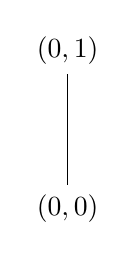
\begin{tikzpicture}
                \node (max) at (2,2) {$(0,1)$};
                \node (min) at (2,0) {$(0,0)$};

                \draw (min) -- (max);
                \draw[preaction={draw=white, -,line width=6pt}] (min) -- (max);
            \end{tikzpicture}
                                        &
            \begin{tikzpicture}
                \node (max) at (0,4) {$(1,1)$};
                \node (a) at (-2,2) {$(1,0)$};
                \node (b) at (2,2) {$(0,1)$};
                \node (min) at (0,0) {$(0,0)$};

                \draw (min) -- (a) -- (max) -- (b);
                \draw[preaction={draw=white, -,line width=6pt}] (a) -- (min) -- (b);
            \end{tikzpicture}
                                        &
            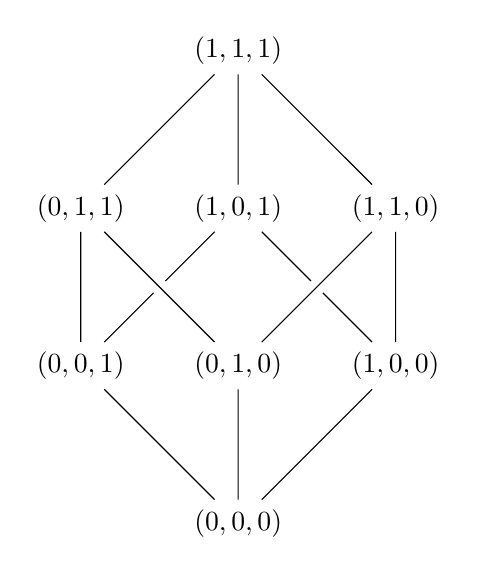
\begin{tikzpicture}
                \node (max) at (0,4) {$(1,1,1)$};
                \node (a) at (-2,2) {$(0,1,1)$};
                \node (b) at (0,2) {$(1,0,1)$};
                \node (c) at (2,2) {$(1,1,0)$};
                \node (d) at (-2,0) {$(0,0,1)$};
                \node (e) at (0,0) {$(0,1,0)$};
                \node (f) at (2,0) {$(1,0,0)$};
                \node (min) at (0,-2) {$(0,0,0)$};
                \draw (min) -- (d) -- (a) -- (max) -- (b) -- (f)
                (e) -- (min) -- (f) -- (c) -- (max)
                (d) -- (b);
                \draw[preaction={draw=white, -,line width=6pt}] (a) -- (e) -- (c);
            \end{tikzpicture}
            \\
            Diagrama Hasse $\mathbb{B}$ & \quad\quad\quad Diagrama Hasse $\mathbb{B}^2$ & \quad\quad\quad Diagrama Hasse $\mathbb{B}^3$
        \end{tabular}
    \end{center}
\end{ejemplo}
\smallskip
\begin{properties}
    Sea $(B, \lor, \land, \overline{\square}, 0, 1)$ un álgebra de Boole. Entonces $\forall x,y,z \in A$:
    \begin{itemize}
        \item $0 \leq x \leq 1$.
        \item Isotonía: Si $x \leq y$, entonces $x \lor z \leq y$ y $x \land z \leq y \land z$.
        \item $x\leq y \Longleftrightarrow \overline{y} \leq \overline{x} \Longleftrightarrow x \leq \overline{y} = 0$.
        \item $x \land y \leq z \Longleftrightarrow x \leq \overline{y} \lor z$.
    \end{itemize}
\end{properties}

\subsection{Átomos de un Álgebra}
\begin{ndef}[Maximal y minimal]
    Sea $X$ un conjunto con una relación de orden $\leq$, y sea $m \in X$. Se dice que $m$ es un \textbf{elemento maximal de $X$}, si y sólo si, no existe $x \in X$ con $x \neq m$ tal que $m \leq x$.
    De manera análoga, $m$ es un \textbf{elemento minimal de $X$}, si y sólo si, no existe $x \in X$ con $m \neq x$ tal que $x \leq m$.
\end{ndef}
\begin{ndef}[Átomo]
    Sea $B$ un álgebra de Boole y $a \in B$. Se dice que $a$ es un \textbf{átomo} si $a$ es un elemento minimal de $B \textbackslash \{0\}$. Es decir,
    $\forall a \in B \textbackslash \{0\} \ (x \leq a \implies x = a)$.
\end{ndef}
\begin{nth}
    Sea $B$ un álgebra de Boole finita y $x \in X \textbackslash \{0\}$. Entonces $x$ se expresa de forma única como supremo de átomos.
\end{nth}
\begin{lema}
    Sea $B$ un álgebra de Boole finita y $x \in X \textbackslash \{0\}$. Entonces existe $a \in B$ átomo tal que $a \leq x$.
\end{lema}
\begin{nota}
    Denotamos por $A_x$ al conjunto de elementos de $A$ menores o iguales que x.
\end{nota}